\documentclass{article}

\usepackage{ctex}
\usepackage{listings}
\usepackage[framed,numbered,autolinebreaks,useliterate]{mcode}
\usepackage{geometry}
\usepackage{graphicx}
\geometry{a4paper, scale=0.8}

\title{数学实验实验报告}
\author{ZhaohengLi 2017050025\\cainetatum@foxmail.com\\15801206130}

\begin{document}

\maketitle{}

\section{实验目的}
\begin{itemize}
	\item{掌握用MATLAB计算拉格朗日、分段线性和三次样条三种插值的方法;}
	\item{掌握在MATLAB中利用梯形公式和辛普森公式计算数值积分;}
	\item{通过实例学习用插值和数值积分解决问题。}
\end{itemize}

\section{计算题}

\subsection{选用3种数值积分方法计算$\pi$}
已知单位圆的面积为$\pi$,则$\pi=2\int_{-1}^{+1}\sqrt{1-x^{2}}$。
\subsubsection{代码实现}
\begin{lstlisting}
X1 = -1 : 2/100 : +1;
X2 = -1 : 2/1000 : +1;
Y1 = 2*sqrt(1-X1.^2);
Y2 = 2*sqrt(1-X2.^2);
PI11 = trapz(X1,Y1);
PI12 = trapz(X2, Y2);

F = @(X) 2*sqrt(1-X.^2);
PI2 = quad(F, -1, +1);
PI3 = quadl(F, -1, +1);

fprintf("当区间个数为100 使用梯形公式得到的结果为:PI=%.15f\n", PI11);
fprintf("当区间个数为1000 使用梯形公式得到的结果为:PI=%.15f\n", PI12);
fprintf("使用辛普森公式得到的结果为:PI=%.15f\n", PI2);
fprintf("使用高斯公式得到的结果为:PI=%.15f\n", PI3);
\end{lstlisting}

\subsubsection{计算结果}
\begin{lstlisting}
当区间个数为100 使用梯形公式得到的结果为:PI=3.138268511098500
当区间个数为1000 使用梯形公式得到的结果为:PI=3.141487477002141
使用辛普森公式得到的结果为:PI=3.141578263238412
使用高斯公式得到的结果为:PI=3.141592066206242
\end{lstlisting}

\subsubsection{结果分析}
三种方法得到的结果均精确到了小数点后第三位。使用梯形公式得到的结果比实际值要小,这是由于算法的固有属性造成的。通过减少区间长度可以缓解这一现象。使用辛普森公式和高斯公式得到的结果更为精确。

\subsection{CH3-T10 机翼剖面}
\subsubsection{算法设计}
题目中仅仅给出了很稀疏的机翼形状边缘的采样点值,因此在进行计算时首先需要对这些点进行插值加密,加密后再进行面积计算。

将机翼剖面的轮廓线分为两段,即y1和y2,分别使用三种方法进行插值,即拉格朗日插值方法、分段线性插值方法和三次样条插值方法。

在计算剖面面积的时候,使用上一步中加密过后的数据点进行数值积分计算,采用了梯形公式和辛普森公式进行面积的计算。
\subsubsection{算法实现}
\begin{lstlisting}
x = [0, 3, 5, 7, 9, 11, 12, 13, 14, 15];
y1 = [0, 1.8, 2.2, 2.7, 3.0, 3.1, 2.9, 2.5, 2.0, 1.6];
y2 = [0, 1.2, 1.7, 2.0, 2.1, 2.0, 1.8, 1.2, 1.0, 1.6];

x_ex = 0 : 0.1 : 15;

y1_ex_lagr = lagr(x, y1, x_ex);
y2_ex_lagr = lagr(x, y2, x_ex);

y1_ex_line = interp1(x, y1, x_ex, 'linear');
y2_ex_line = interp1(x, y2, x_ex, 'linear');

y1_ex_spli = interp1(x, y1, x_ex, 'spline');
y2_ex_spli = interp1(x, y2, x_ex, 'spline');

disp(x_ex);
disp(y1_ex_lagr);

figure;
subplot(3,1,1);
title("lagr");
hold on;
scatter(x, y1);
scatter(x, y2);
plot(x_ex, y1_ex_lagr);
plot(x_ex, y2_ex_lagr);

subplot(3,1,2);
title("linear");
hold on;
scatter(x, y1);
scatter(x, y2);
plot(x_ex, y1_ex_line);
plot(x_ex, y2_ex_line);

subplot(3,1,3);
title("spline");
hold on;
scatter(x, y1);
scatter(x, y2);
plot(x_ex, y1_ex_spli);
plot(x_ex, y2_ex_spli);

S11 = trapz(x_ex, y1_ex_lagr) - trapz(x_ex, y2_ex_lagr);
S12 = trapz(x_ex, y1_ex_line) - trapz(x_ex, y2_ex_line);
S13 = trapz(x_ex, y1_ex_spli) - trapz(x_ex, y2_ex_spli);

S21 = simpson(x_ex, y1_ex_lagr) - simpson(x_ex, y2_ex_lagr);
S22 = simpson(x_ex, y1_ex_line) - simpson(x_ex, y2_ex_line);
S23 = simpson(x_ex, y1_ex_spli) - simpson(x_ex, y2_ex_spli);

\end{lstlisting}

\begin{lstlisting}
function [ integral ] = simpson( X, Y )

%simpson: Calculate the integral using simpson formula % Input X and Y are discrete values of y = f(x)
% X is supposed to be evenly distributed.
% Notice that length(X)=length(Y) must be odd.

m = (length(X) -1) / 2;
h = (max(X) - min(X)) / (2 * m);
integral = Y(1) + Y(2 * m + 1) + 4 * Y(2);
for k = 1:(m - 1)
    integral = integral + 4 * Y(2 * k + 2) + 2 * Y(2 * k + 1);
end
integral = integral * h / 3;
end
\end{lstlisting}

\subsubsection{计算结果}

首先是数据点加密的过程,三种加密方式结果如图中所示。

\begin{figure}[htb]
    \centering
    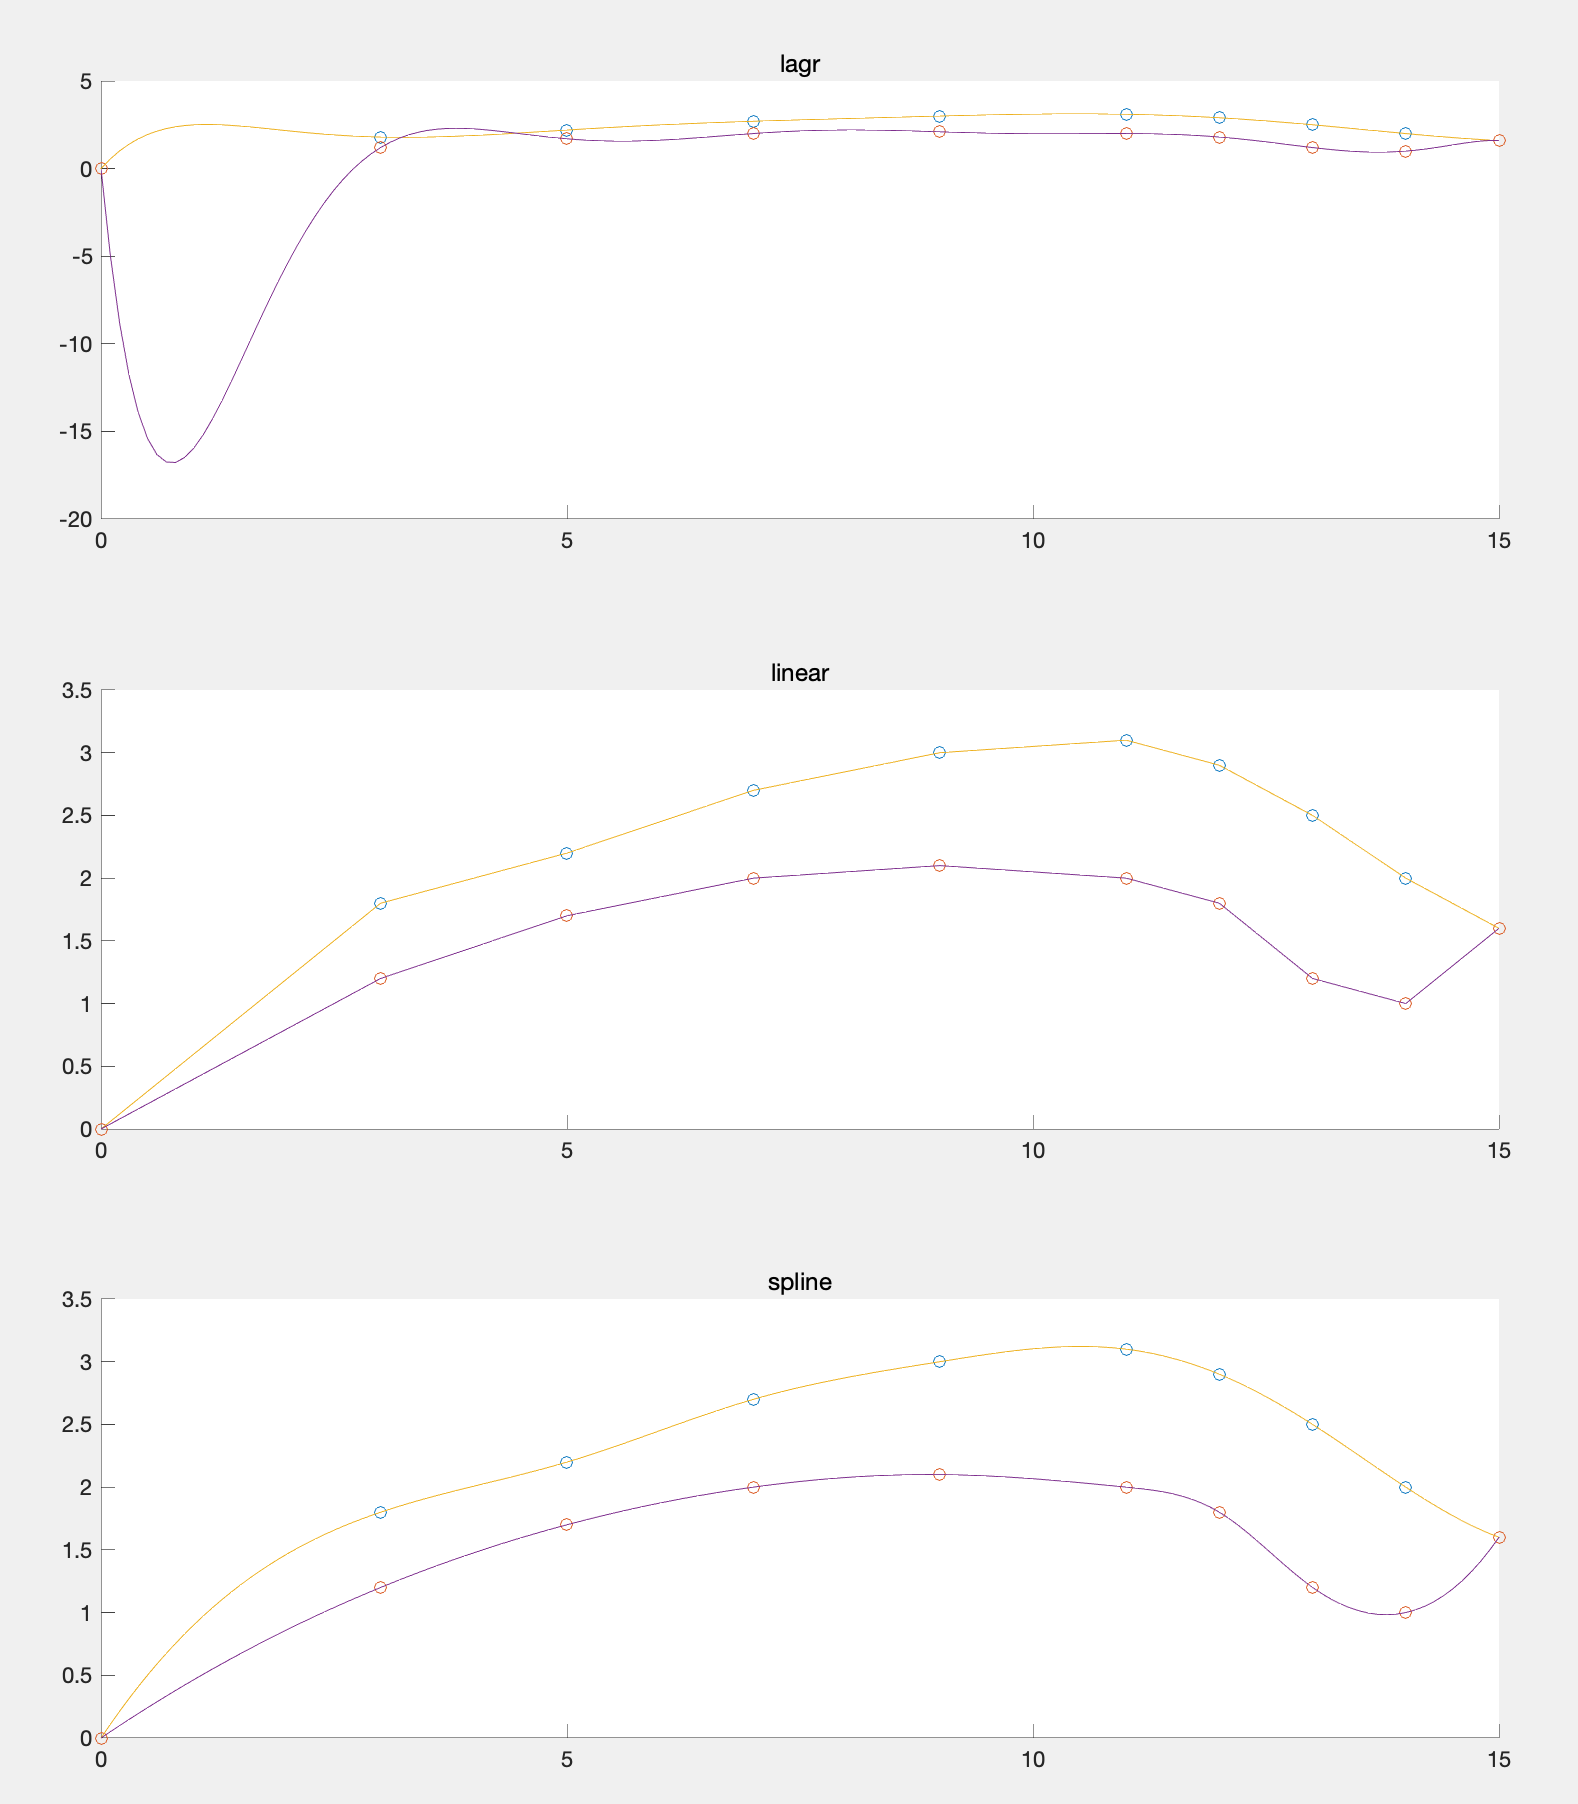
\includegraphics[width=0.7\textwidth]{pic1.png}
    \caption{数据点加密后的图像}
\end{figure}

对加密后的数据点进行梯形公式数值积分和辛普森公式数值积分结果如表中所示。

\begin{table}[htb]
	\centering
	\caption{数值积分结果}
	\begin{tabular}{ccc}
\hline
插值方法 & 梯形公式计算的面积 & 辛普森公式计算的面积 \\
 \hline
拉格朗日插值法 & 40.3044 & 40.3553 \\ 
分段线性插值法 & 10.7500 & 11.3444 \\
三次样条插值法 & 10.7500 & 11.3460 \\
\hline
\end{tabular}
\end{table}

\subsubsection{结果分析}

从结果中可以看出,使用拉格朗日线性插值法出现了“Runge现象”,曲线震荡非常 严重,不能作为加工的曲线使用,同时使用拉格朗日插值之后的数据点来进行面积计算 时也有很大的偏移,不适合在该问题中使用。
而分段线性插值和样条插值法给出的加工数据则更加合理,二者拟合的曲线也比较相近, 但是如果需要用在工业生产中,还是样条插值给出的曲线更加平滑,能够给予机翼更好的流 线,应该在该问题中被采用。
至于梯形公式和辛普森积分公式的面积计算,从结果上看二者表现相近,差距不大。
\subsubsection{结论}

在计算机翼加工断面的面积时,应该先选用三次样条加密数据点,在使用辛普森公式计算数值积分。在本题中,加工面积为11.34。

\newpage
\section{应用题}

\subsection{问题分析}
本题要求估算一天的车流量,但是并未给出每分钟的车流量,必须要设法求出或估计出其他各个时刻的车流量分布,才能计算出一天的车流量。
\subsection{模型假设与建立}
将车流量抽象为关于时间的函数$f(t)$,函数值表示在$t_{i}$到$t_{i+1}$这段时间内通过桥梁的车辆数。显然有 $f(t)\geq0, \forall t \geq 0$。为更加符合实际意义,在此给出一些约束:
\begin{itemize}
	\item{约束一:$f$是关于$t$的连续函数}
	\item{约束二:$f$的二阶导数连续(保证车流变化的连续性)}
\end{itemize}
因此本题的目标为在约束条件下求解:$$\int_{t_{start}}^{t_{end}}f(t)dt$$
\subsection{算法设计与实现}
在仅考虑约束一的条件下,仅需要利用当前已经给出的数据点使用梯形公式进行数值积分即可。在考虑两个约束的条件下,需要先试哟哦那个三次样条差值方法加密数据点,在使用梯形公式进行数值积分。
\begin{lstlisting}
x = [0 2 4 5 6 7 8 9 10.5 11.5 12.5 14 16 17 18 19 20 21 22 23 24] * 60;
y = [2 2 0 2 5 8 25 12 5 10 12 7 9 28 22 10 9 11 8 9 3];
sum1 = trapz(x,y);
x_ex = 0 : 24*60;
y_ex = interp1(x, y, x_ex, 'spline');
sum2 = trapz(x_ex, y_ex);
figure;

subplot(2,1,1);
plot(x, y);
xlabel("Time/min");
ylabel("Cars");
title("满足约束一");


subplot(2,1,2);
plot(x_ex, y_ex);
xlabel("Time/min");
ylabel("Cars");
title("满足约束一和约束二");

\end{lstlisting}
\subsection{结果计算与分析}
不同约束条件下汽车流量如图所示,由于取样的数据点较少,所以给出的车流量估计值的精确性会受到一定影响。

在约束一的条件下,计算的车流量为12990辆;在约束一和约束二的条件下,计算的车流量为12668辆。
\begin{figure}[htb]
    \centering
    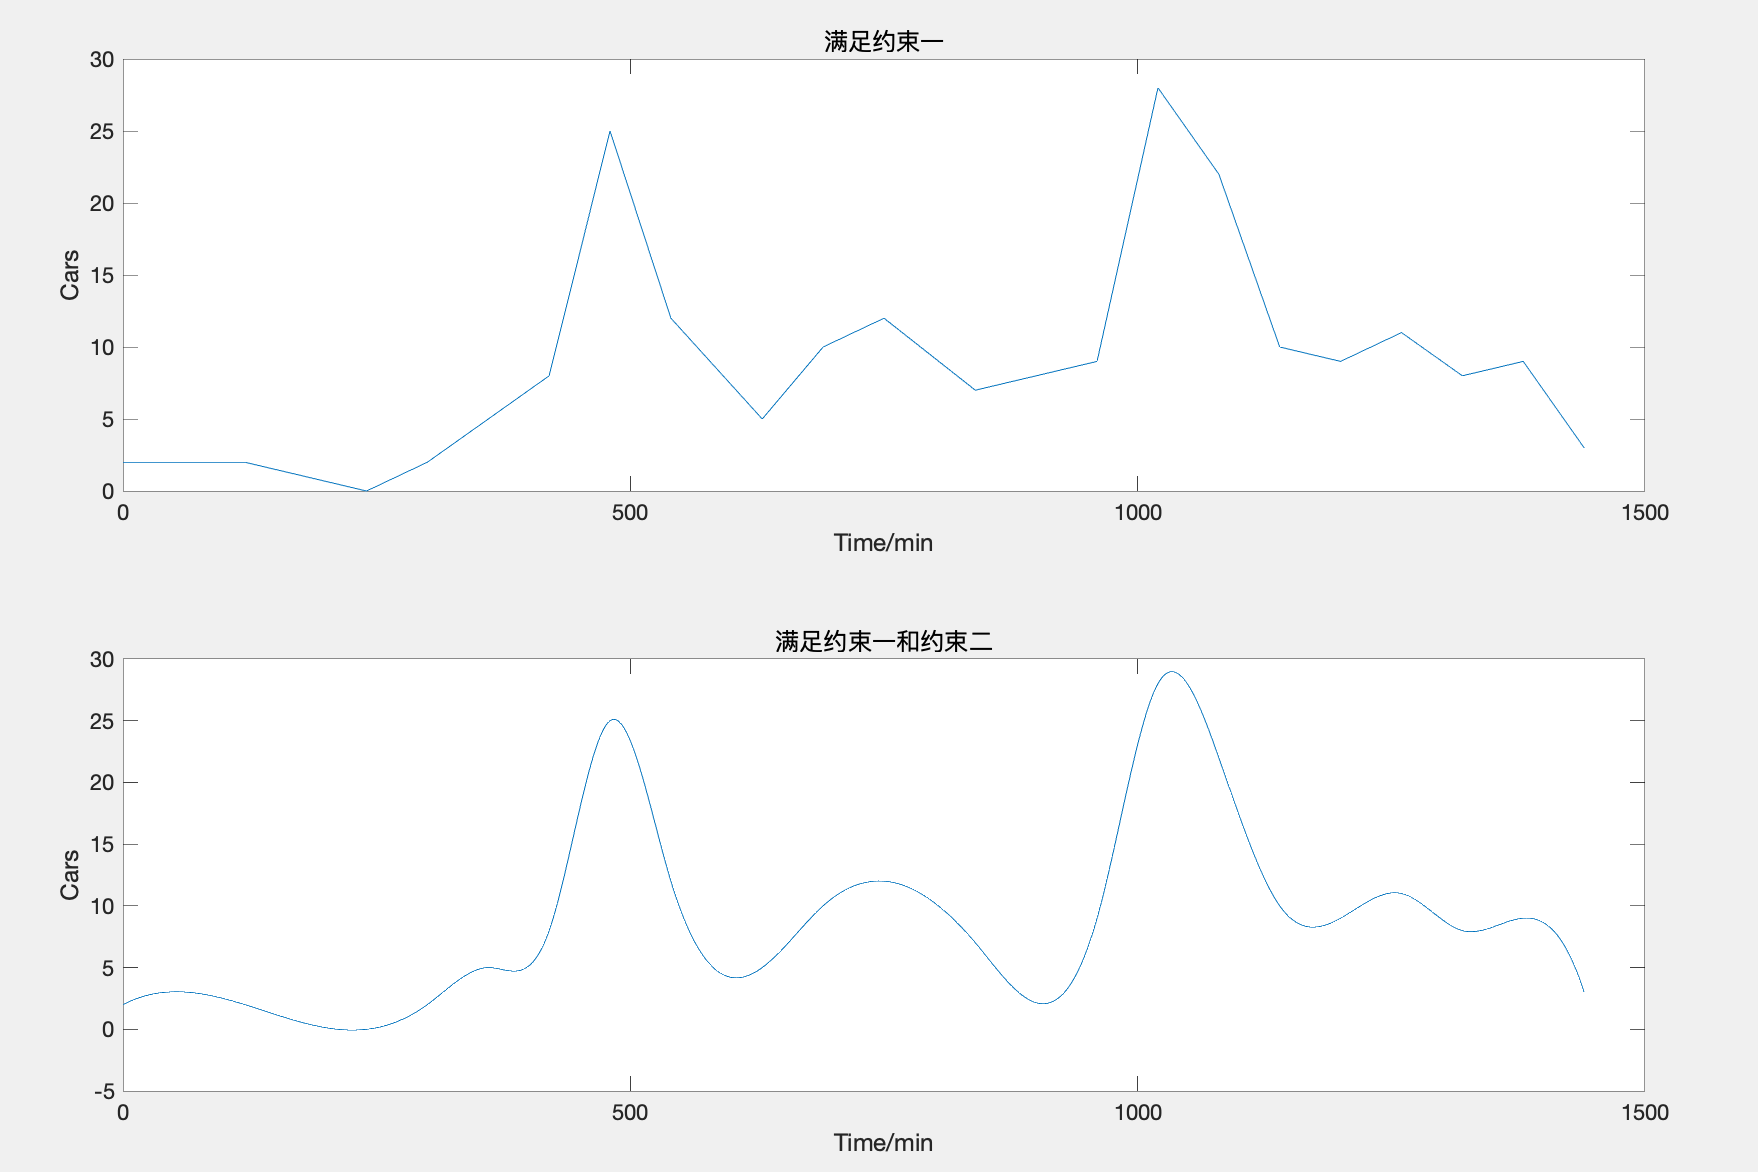
\includegraphics[width=0.7\textwidth]{pic2.png}
    \caption{数据点加密后的图像}
\end{figure}

\subsection{结论}
在该模型下,一天通过桥梁的车流量大约为1.2-1.3万辆左右。

\section{收获与建议}

通过这次的实验,我对MATLAB中提供的插值函数和数值积分函数理解更加深刻,通过画图的方式观察并体会了不同方式的差别与优缺点,同时在做实验的过程中,我对MATLAB的使用也更加熟练了。希望在之后的课堂上老师可以指出我们设计模型和算法中忽略的细节让我们加以改正。

\end{document}